\section{Inteligência Artificial}

\subsection{Cobra}

A cobra rasteja aleatoriamente no cenário. A partir do momento que
Medrash entra no campo de deteção da cobra, esta fica em posição
de ataque. Se Medrash se aproximar ainda mais, ela o atacará.
A única forma de Medrash evitar este ataque será esquivando. O ataque
ignora a defesa de Medrash.
Uma vez que Medrash saia se afaste do campo de deteção da cobra, ela
voltará a patrulhar.

\begin{center}
 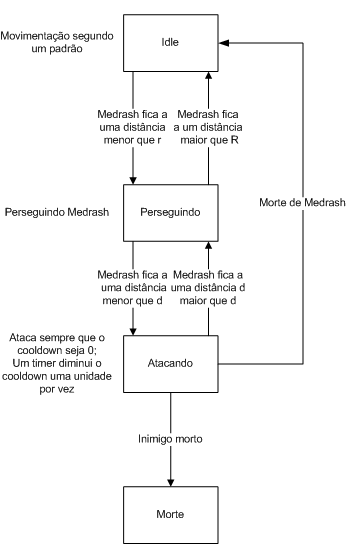
\includegraphics[scale=1]{ia_simples.png}
 %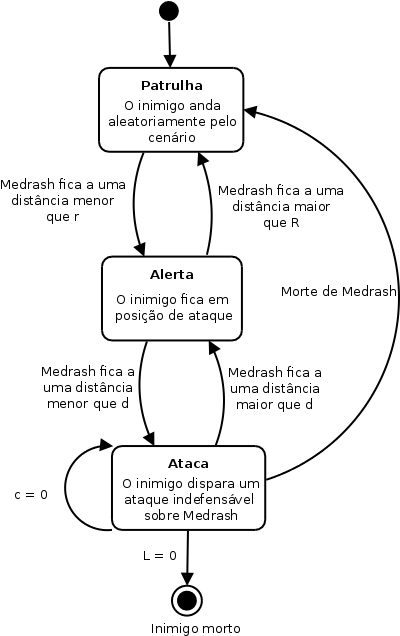
\includegraphics[scale=1]{ia_cobra.png}
\end{center}

\subsection{Enxame de abelhas}

O enxame de abelhas fica aglomerado na colméia. Quando Medrash se
aproxima o suficiente da colméia, o enxame começa a perseguí-lo.
A única opção de Medrash é fugir, pois as abelhas não podem ser atacadas.
Quando Medrash se afastar o suficiente da colméia, o enxame deixa
de perseguí-lo.
Se o enxame se aproximar de Medrash, irá atacá-lo.

\begin{center}
 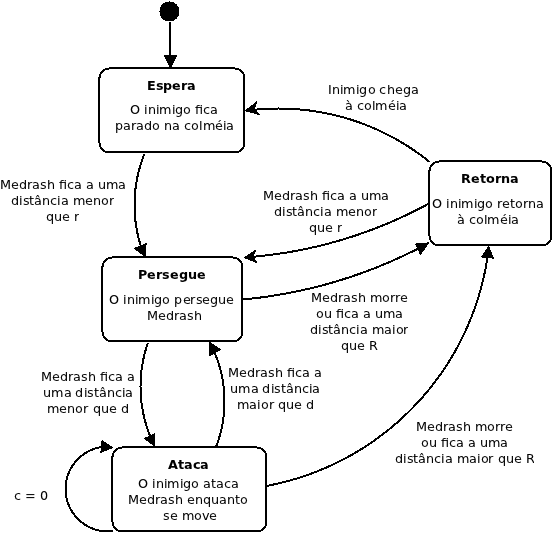
\includegraphics[scale=0.7]{ia_enxame.png}
\end{center}

\subsection{Jacaré}

O jacaré fica nas proximidades do rio. Se Medrash se aproximar dele,
este o perseguirá. Se Medrash se afastar o suficiente dele, o jacaré voltará às proximidades de seu ponto inicial.
O jacaré se movimenta dentro e fora do rio. Caso ele fique próximo de
Medrash, irá atacá-lo. Se sua barra de vida estiver baixa, ele atacará
múltiplas vezes.

\begin{center}
 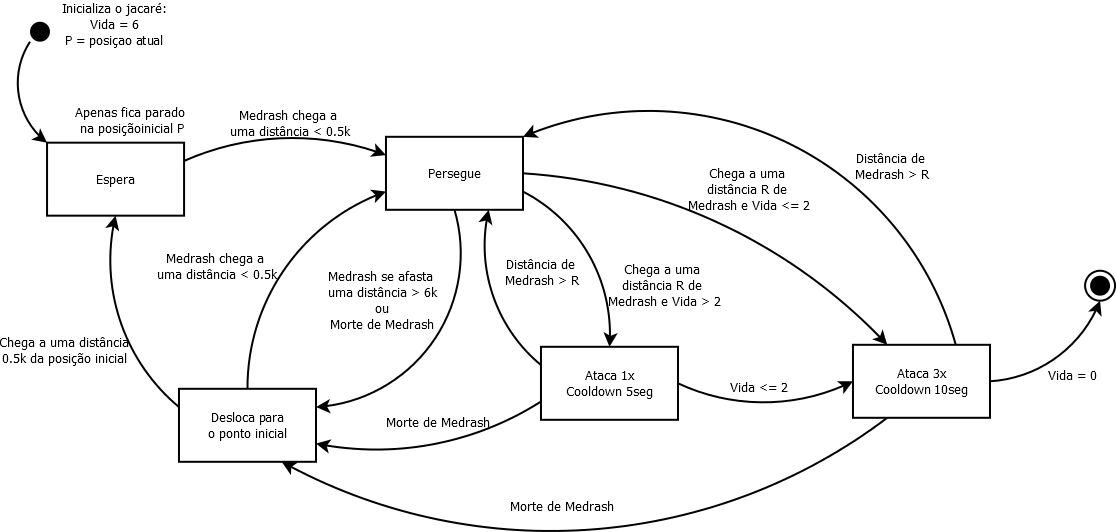
\includegraphics[scale=0.4]{ia_jacare.png}
\end{center}

\subsection{Tigre (1$^\circ$ chefe)}

Sendo o chefe da primeira fase, o tigre segue uma estratégia mais agressiva.
Inicialmente, ele corre em volta de Medrash, mantendo-se à uma distância
 segura. Após algum tempo, ele correrá em direção ao Medrash. Caso se
 aproxime, ele o atacará. Se Medrash conseguir se afastar por tempo
 suficiente, o tigre voltará a circular Medrash.
Periodicamente o tigre andará devagar para recuperar sua energia. Nesse
período, o Medrash consegue alcança-lo, e atacá-lo. Ao ser atacado, o tigre
volta a circular.
Quando sua barra de vida estiver baixa, o tigre também irá preparar um
bote. Ele ficará esperando Medrash se aproximar. Caso Medrash se aproxime,
 ele atacará com um salto. Se Medrash permanecer afastado por tempo 
suficiente, ele voltará a circular.

\begin{center}
 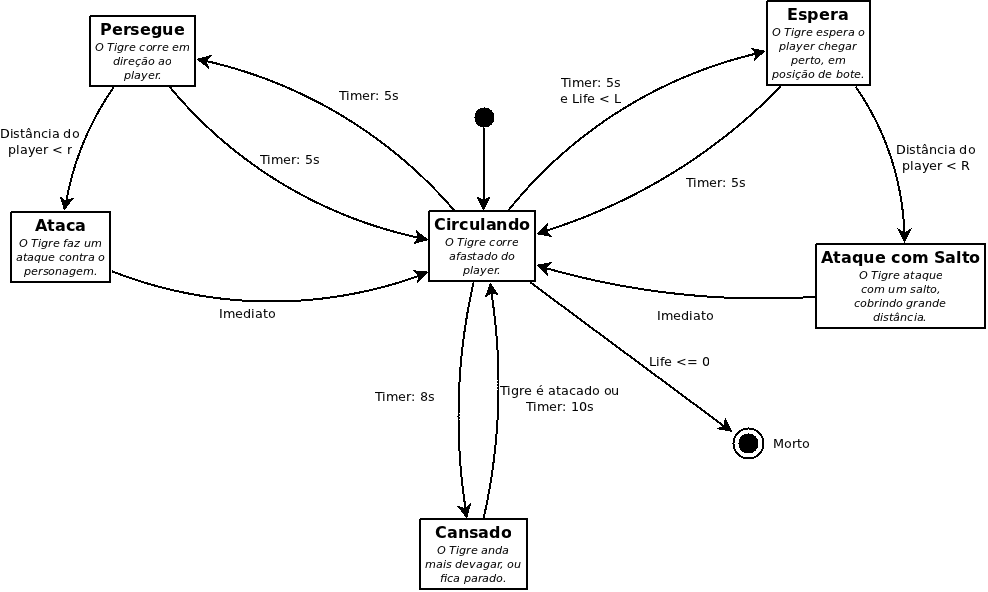
\includegraphics[scale=0.5]{ia_tigre.png}
\end{center}

\subsection{Urso}

O urso fica patrulando na floresta. Caso Medrash entre no raio de deteção
do urso, este o perseguirá. Para fugir do urso, Medrash deve ficar a uma
distância bem maior que o raio de deteção.
Se o urso se aproximar muito de Medrash, este será atacado. Enquanto estiver
próximo, o urso, periodicamente, irá se defender.

\begin{center}
 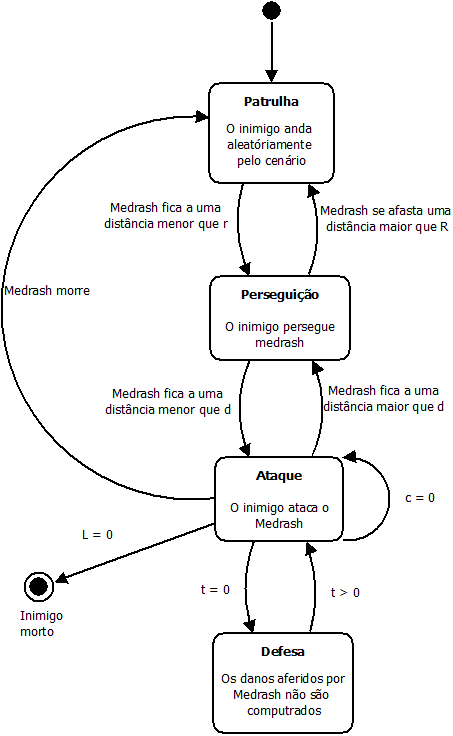
\includegraphics[scale=0.5]{ia_urso.png}
\end{center}
